\subsubsection{Introduction}
The database should contain all necessary tables for fetching, storing and displaying TV-shows and their episodes, as well as all attributes related to these that may be of interest to the user, such as original pilot date, amount of episodes, and details for each episode. 

There must also be supporting tables, such as \textit{country}, \textit{roles} and \textit{channel} which must exist for the database to be in 3NF and allow values to be atomic. To allow a \textit{user} to mark whether he or she is actually watching a \textit{show}, relational tables such as \textit{user\_show} must also be created, and for a future administration interface, \textit{parameter} needs to exist for storing and managing site-wide configuration without manually editing the configuration file.

Furthermore, additional functionality which has not yet been fully implemented must be supported by the database, i.e tables \textit{url} and \textit{subtitle}, which are meant to contain links to where a specific episode can be watched or downloaded, as well as where subtitles may be found. 

\subsubsection{Logical design model}

\begin{description}
	\item[actor] (actor\_id, imdb\_id, poster\_url, name)
		\begin{description}
			\item[Primary Key] actor\_id
		\end{description}
	\item[channel] (id, name, country\_id)
		\begin{description}
			\item[Primary Key] id
			\item[Foreign Keys] \hfill \\ country\_id \textbf{references} country(id)
		\end{description}	
	\item[country] (id, name, language)
		\begin{description}
			\item[Primary Key] id
		\end{description}
	\item[episode] (show\_id,season,episode,name,summary,date)
		\begin{description}
			\item[Primary Key] show\_id, season, episode
			\item[Foreign Keys] \hfill \\ show\_id \textbf{references} show(id)
		\end{description}
	\item[parameter] (id,key,value )
		\begin{description}
			\item[Primary Key] id
		\end{description}
	\item[roles] (id,name,description,is\_admin)
		\begin{description}
			\item[Primary Key] id
		\end{description}
	\item[show] (id,imdb\_id,zap2\_id,channel\_id,poster,pilot\_date,name,summary,lang,rating,lst\_update)
		\begin{description}
			\item[Primary Key] id
		\end{description}
	\item[subtitle] (show\_id,season,episode,url )
		\begin{description}
			\item[Primary Key] show\_id, season, episode
			\item[Foreign Keys] \hfill \\ show\_id \textbf{references} show(id) \hfill \\ season \textbf{references} episode(season) \hfill \\ episode \textbf{references} episode(episode)
		\end{description}
	\item[url] (show\_id,season,episode,url)
		\begin{description}
			\item[Primary Key] show\_id, season, episode
			\item[Foreign Keys] \hfill \\ show\_id \textbf{references} show(id) \hfill \\ season \textbf{references} episode(season) \hfill \\ episode \textbf{references} episode(episode)
		\end{description}
	\item[user] (id,email,password,salt,role\_id,country\_id,last\_activity)
		\begin{description}
			\item[Primary Key] id
			\item[Foreign Keys] \hfill \\ role\_id \textbf{references} roles(id) \hfill \\ country\_id \textbf{references} country(id)
		\end{description}
	\item[user\_session] (id,session\_data,session\_ip)
		\begin{description}
			\item[Primary Key] id
		\end{description}
	\item[user\_show] (user\_id,show\_id,is\_favorite  )
		\begin{description}
			\item[Foreign Keys] \hfill \\ show\_id \textbf{references} show(id) \hfill \\ user\_id \textbf{references} user(id)
		\end{description}
	
\end{description}
	
\subsubsection{Entity-Relationship Diagram}
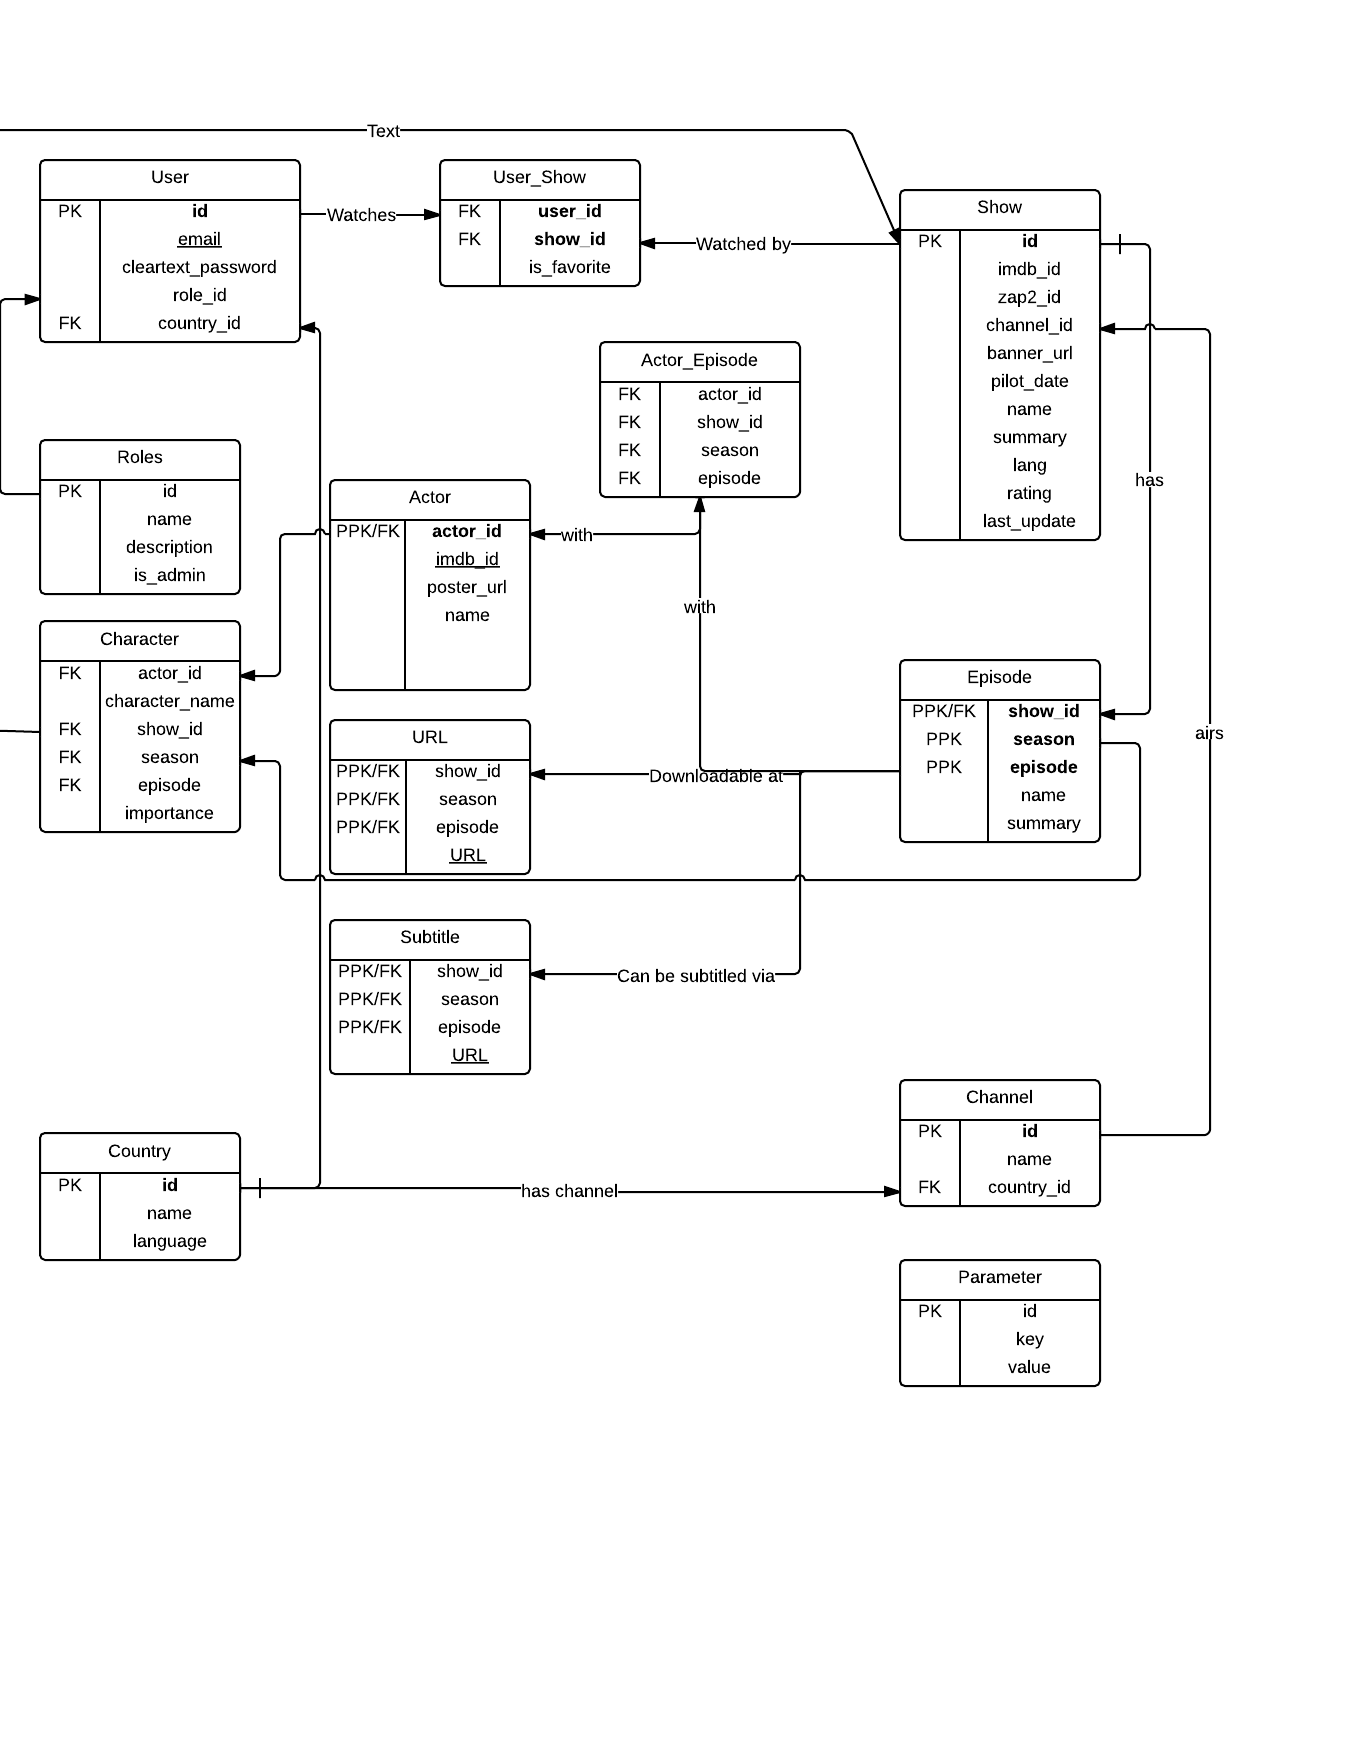
\includegraphics[scale=0.39]{erd}